\chapter{Análise Teórica}
\label{ch:anal_teo} % This how you label a chapter and the key (e.g., ch:into) will be used to refer this chapter ``Introduction'' later in the report. 
% the key ``ch:into'' can be used with command \ref{ch:intor} to refere this Chapter.

\section{Bubble Sort} 

\section{Merge Sort}

Desenvolvido por \href{https://en.wikipedia.org/wiki/John_von_Neumann}{Jon Von Neumann} em 1945, o Merge Sort é um algoritmo de \href{https://en.wikipedia.org/wiki/Divide-and-conquer_algorithm}{dividir para conquistar}, que subdivide uma lista em singletons e os mescla em sublistas ordenadas até que exista apenas uma sublista, esta sublista é a lista original ordenada. Imagine o seguinte caso:

Você tem um baralho de cartas e gostaria de organizá-lo, seguindo o conceito do Merge Sort você trabalha da seguinte forma:
\begin{itemize}
  \item \textbf{Divisão:} Primeiro você divide o baralho em dois baralhos menores. Cada um desses baralhos é dividido novamente até que cada sub-baralho tenha uma carta.
  \item \textbf{"Merge" (Mescla):} Nesse momento, com cada sub-baralho com uma carta, todos estão ordenados, então você começa a juntar os sub-baralhos comparando duas cartas de cada baralho e colocando-as em ordem crescente. Assim dois grupos de uma carta se tornam um baralho de duas cartas ordenadas. Em seguida, dois baralhos de duas cartas são mesclados para formar um baralho de quatro cartas, e assim por diante, até que todas as cartas estejam combinadas novamente, mas agora ordenadas.
\end{itemize}
\begin{figure}[!ht]
    \centering
    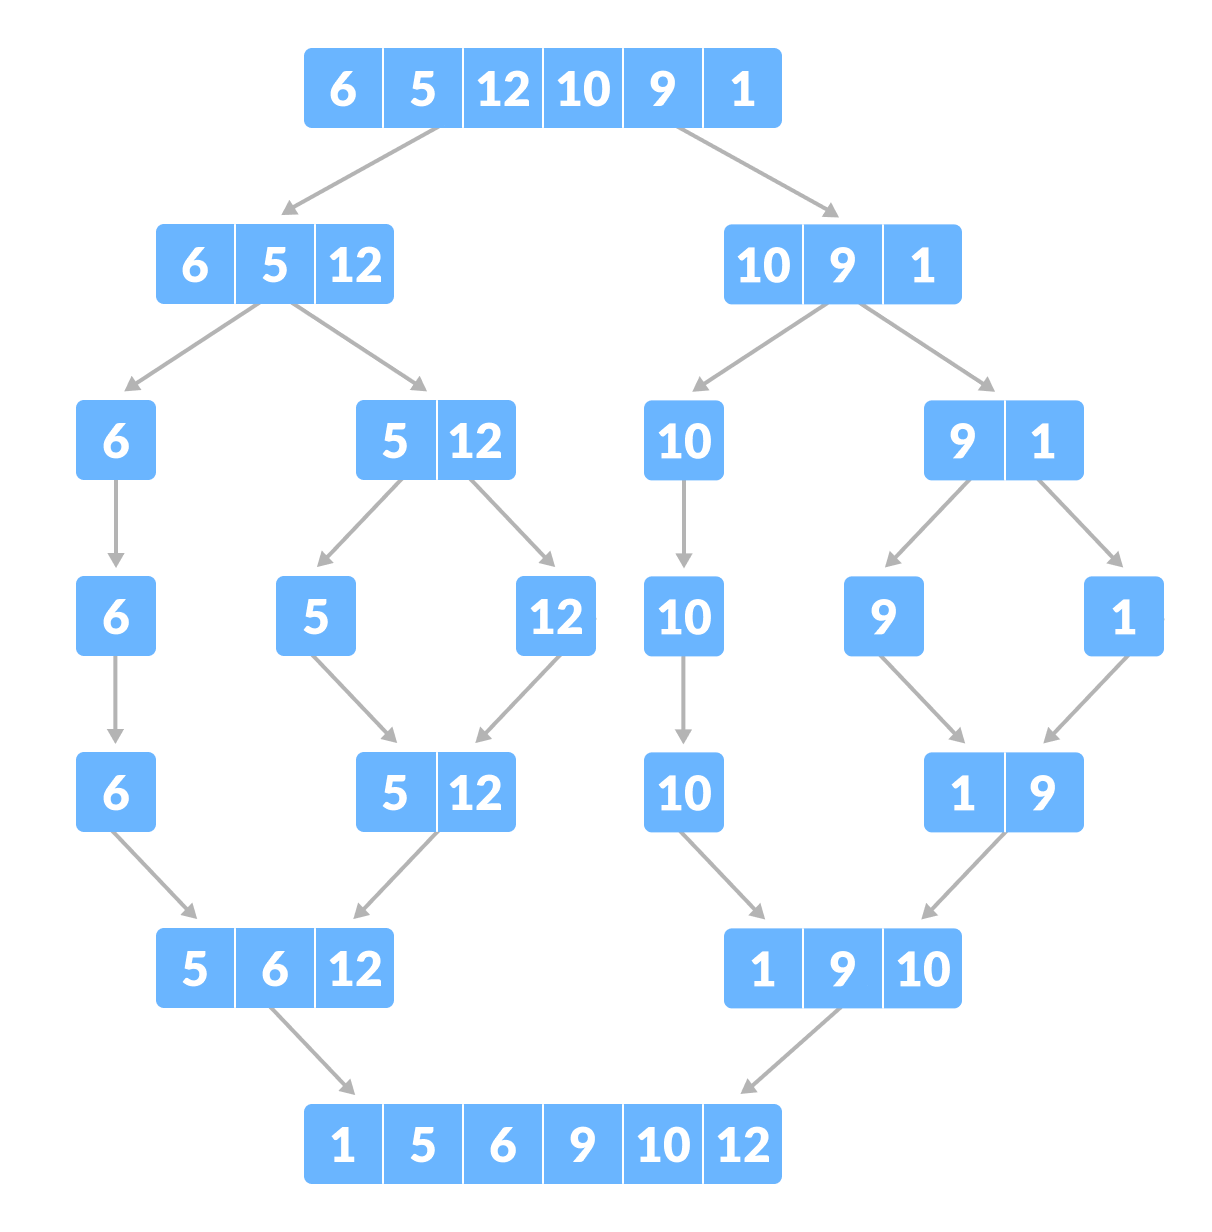
\includegraphics[scale=0.3]{figures/merge-sort-example_0.png}
    \caption{Diagrama exemplo de um Merge Sort}
    \label{fig:merge_sort_example_0}
\end{figure}

\noindent
Dito isso, o pseudocódigo desse algoritmo na forma recursiva pode ser escrito como:

\begin{algorithm}
    \label{algo:merge_sort_pseudo}
    \begin{algorithmic}[1]
        \Require{$ \mathbf{lista}  = x_1, x_2, \ldots, x_N$}
        \Ensure{A lista ordenada}
        \Statex
        \Function{MergeSort}{$\mathbf{lista}$}
        \If{\textbf{lista} tem um elemento} \Comment Uma lista com um elemento está ordenada
        \State \Return
        \EndIf
        \State {MergeSort(primeira metade da \textbf{lista})}
        \State {MergeSort(segunda metade da \textbf{lista})}
        \State {Merge(\textbf{lista}, primeira metade da \textbf{lista}, segunda metade da \textbf{lista})}
        \EndFunction
    \end{algorithmic}
\end{algorithm}
 

%  TODO:
% - Pseudocódigo
% - Análise de complexidade


\section{Quick Sort}

